\documentclass[11pt,letterpaper]{article}
\usepackage[margin=1in]{geometry}
\usepackage[T1]{fontenc}
\usepackage{newtxtext,newtxmath}
\usepackage{graphicx,booktabs,xcolor,amsmath,microtype,tikz,enumitem,caption,array}
\usepackage[hidelinks]{hyperref}
\usetikzlibrary{positioning,fit,arrows.meta,calc,backgrounds,decorations.pathreplacing}
\captionsetup{font=small,labelfont=bf}
\setlist{itemsep=2pt,topsep=4pt,leftmargin=1.4em}
\setlength{\parskip}{4pt}
\definecolor{cblue}{HTML}{2a78d6}
\definecolor{corange}{HTML}{eb6834}
\definecolor{caqua}{HTML}{1baf7a}
\definecolor{cpurple}{HTML}{8c5bd6}
\definecolor{cgray}{HTML}{8a8984}
\newcommand{\code}[1]{\texttt{\small #1}}
\newcommand{\shape}[1]{\texttt{\footnotesize[#1]}}
\tikzset{
  arr/.style={-{Stealth[length=5pt]},draw=black!60,thick},
  box/.style={draw=#1!80!black,fill=#1!10,rounded corners=2pt,inner sep=4pt,align=center},
  box/.default=cgray,
}

\title{\Large\bfseries One Network for Picks and Wheels\\[2pt]\large The architecture of a combined PickNet + WheelNet}
\author{Design note. Companion to \emph{How PickNet Works} and \emph{How WheelNet Works}}
\date{\small October 2026 \quad\textperiodcentered\quad Status: proposed; frozen probe implemented, full run pending}

\begin{document}
\maketitle

\noindent PickNet predicts which card a drafter takes. WheelNet predicts which of the cards they pass will
come back eight picks later. The two models read almost the same input, and they are built from the same
parts: a card table, a causal history encoder over one token per pick, and a decoder over the cards in a
pack. This note describes one network that does both jobs: a shared trunk with a \emph{pick head} and a
\emph{wheel head}. It reuses the terms of the two companion guides (history token $\mathbf x_t$, history
state $\mathbf h_t$, candidate token, passed-card token, bag, draft context, wheel-eligible pick), and only
explains what is new. Code: \code{scripts/probe\_picknet\_wheel.py} in the wheelnet repo (the frozen probe,
Section~\ref{sec:plan}); the trunk is \code{PickNet} in \code{picknet/src/picknet/model.py}.

{\small\setlength{\parskip}{0pt}\tableofcontents}

% =====================================================================
\section{The job, and why one network}

For every draft, the combined network outputs two things in one forward pass:

\begin{enumerate}
\item \textbf{Pick probabilities} at every slot: a softmax over the cards in pack $t$, exactly as PickNet.
\item \textbf{Wheel probabilities} at every wheel-eligible pick: for each distinct card passed at $t$, the
probability that at least one copy is still in the pack when it returns at $t+8$, exactly as WheelNet.
\end{enumerate}

There are three reasons to expect sharing to work, roughly in order of strength.

\begin{itemize}
\item \textbf{A wheel is seven picks.} A card wheels if each of the next seven drafters passes it. That is
seven pick decisions by people the model cannot see but can infer from what they took. A model that has
learned how drafters pick already holds most of what a wheel model needs: how strong each card is in this
format, which cards protect each other in a pack, and which colours the table is taking.
\item \textbf{Same input, same labels source.} Both models read the packs shown, the picks made and what
the others took, and both get their labels from the same 17Lands rows. Every draft gives pick labels at all
42 slots and wheel labels for 189 passed cards (18 wheel-eligible picks, 13 down to 8 passed cards
each).
\item \textbf{One model to run live.} The overlay in the project's open list wants ``what should I take''
and ``what will come back'' at the same moment. Section~\ref{sec:counterfactual} shows the combined network
can also answer the question a drafter actually asks: \emph{if I take A, will B wheel?}
\end{itemize}

What we expect: the wheel task gains (it gets a much better-trained card and history representation) and
the pick task gains little or nothing. The pick task is the flagship, so the design treats any loss of pick
accuracy as a failure (Section~\ref{sec:loss}).

% =====================================================================
\section{The big picture}

\begin{figure}[!htbp]
\centering
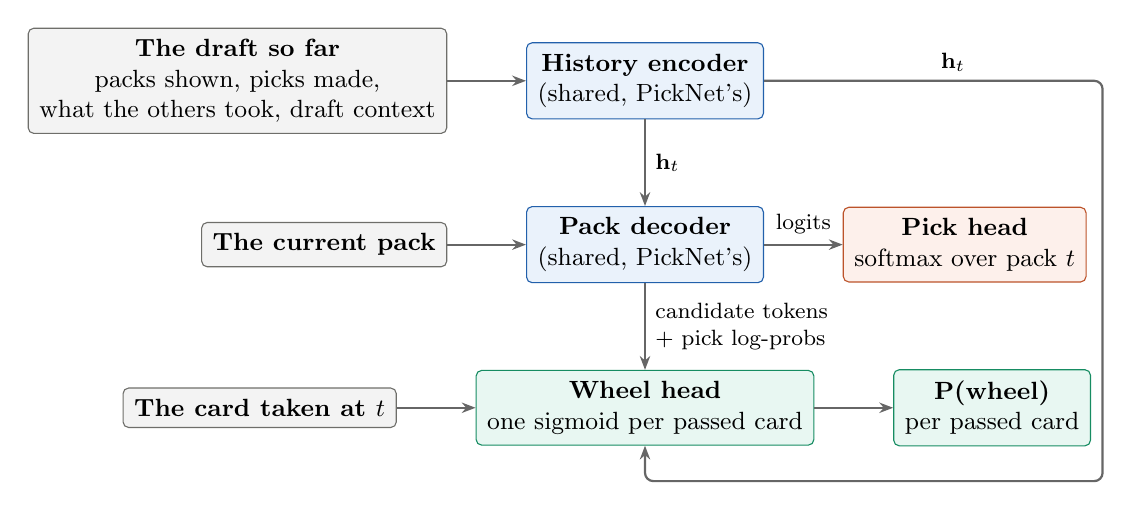
\begin{tikzpicture}[font=\small,node distance=0.55cm]
\node[box] (data) {\textbf{The draft so far}\\packs shown, picks made,\\what the others took, draft context};
\node[box=cblue,right=1.0cm of data] (hist) {\textbf{History encoder}\\(shared, PickNet's)};
\node[box=cblue,below=1.1cm of hist] (dec) {\textbf{Pack decoder}\\(shared, PickNet's)};
\node[box,left=1.0cm of dec] (pack) {\textbf{The current pack}};
\node[box=corange,right=1.0cm of dec] (pick) {\textbf{Pick head}\\softmax over pack $t$};
\node[box=caqua,below=1.1cm of dec] (wheel) {\textbf{Wheel head}\\one sigmoid per passed card};
\node[box,left=1.0cm of wheel] (took) {\textbf{The card taken at $t$}};
\node[box=caqua,right=1.0cm of wheel] (pw) {\textbf{P(wheel)}\\per passed card};
\draw[arr] (data) -- (hist);
\draw[arr] (hist) -- node[right,font=\footnotesize]{$\mathbf h_t$} (dec);
\draw[arr] (pack) -- (dec);
\draw[arr] (dec) -- node[above,font=\footnotesize]{logits} (pick);
\draw[arr] (dec) -- node[right,font=\footnotesize,align=left]{candidate tokens\\+ pick log-probs} (wheel);
\draw[arr] (took) -- (wheel);
\draw[arr] (wheel) -- (pw);
\draw[arr,rounded corners=3pt] (hist.east) -- ++(4.3,0) |- ([yshift=-0.45cm]wheel.south) -- (wheel.south);
\node[font=\footnotesize,anchor=south] at ([xshift=2.4cm]hist.east) {$\mathbf h_t$};
\end{tikzpicture}
\caption{The combined network. Blue: PickNet's trunk, unchanged. Orange: PickNet's own scoring head.
Green: the new wheel head. The card taken at $t$ enters only the wheel head (Section~\ref{sec:timing}).}
\label{fig:big}
\end{figure}

The trunk is PickNet with nothing changed: card table, history tokens, causal history encoder, pack
decoder. The pick head is PickNet's scoring head. The only new part is the wheel head, a small network that
reads the trunk's outputs at a wheel-eligible pick $t$ and scores each passed card.

The wheel head does \emph{not} get its own history encoder or its own pack decoder. That is the point of the
design: all of WheelNet's 4 history layers and 3 decoder layers are replaced by PickNet's.

% =====================================================================
\section{The one real problem: when does the pick happen?}\label{sec:timing}

PickNet and WheelNet disagree about one detail of the history token, and everything in the design follows
from it.

\begin{center}\small
\begin{tabular}{lll}
\toprule
& PickNet token $t$ & WheelNet token $t$ \\
\midrule
pack shown & pack $t$ & pack $t$ \\
card taken & at $t-1$ (\code{pick\_in(prev)}) & at $t$ (\code{taken(card(pick))}) \\
state $\mathbf h_t$ knows & every pick \emph{before} $t$ & every pick \emph{up to and including} $t$ \\
\bottomrule
\end{tabular}
\end{center}

Both are right for their job. PickNet predicts pick $t$, so pick $t$ must not be in its own state. WheelNet
scores the cards \emph{passed} at $t$, which only exist once pick $t$ is made, and which card you took matters
(take the only red card and the remaining cards look different to the table).

So a shared trunk can't simply reuse WheelNet's convention: that would hand the pick head its own answer.
The options are:

\begin{enumerate}
\item \textbf{Read pick $t$ in the wheel head only (chosen).} Keep PickNet's trunk exactly as it is. The
wheel head receives $\mathbf h_t$, the candidate tokens of pack $t$, and the card vector $\mathbf e_{\text{pick}_t}$
as a separate input. The trunk never sees pick $t$ at slot $t$; the wheel head does.
\item \textbf{Read state $\mathbf h_{t+1}$.} PickNet's next state does contain pick $t$. But it also
contains pack $t+1$, which you do not have when you decide what to pass, so the live overlay could not use
it. It also moves the wheel head one slot closer to the label (below).
\item \textbf{Two history streams.} Run the history encoder twice, with and without pick $t$. This doubles
the trunk's cost and gives up the efficiency that motivated sharing.
\end{enumerate}

Option 1 has a bonus: since pick $t$ is a separate input to a small head, the head can be re-run with a
different pick for almost no cost (Section~\ref{sec:counterfactual}).

\subsection{Where the wheel label hides, and the leakage rule}

The label for a card passed at pick $p$ is the pack shown at pick $p+8$. That pack is an input to history
token $p+8$, and the others-taken bag of token $p+8$ is literally ``passed at $p$ minus what came back''.
In a model that reads the whole draft in one pass, this is the main way to fool yourself.

\begin{figure}[!htbp]
\centering
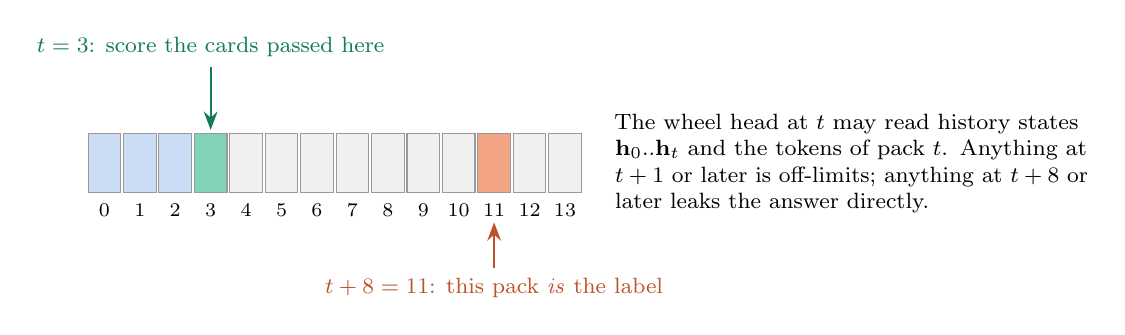
\begin{tikzpicture}[font=\scriptsize,x=0.45cm,y=0.5cm]
\foreach \i in {0,...,13} {
  \ifnum\i<3 \fill[cblue!25] (\i,0) rectangle ++(0.92,1.5);
  \else\ifnum\i=3 \fill[caqua!55] (\i,0) rectangle ++(0.92,1.5);
  \else\ifnum\i=11 \fill[corange!60] (\i,0) rectangle ++(0.92,1.5);
  \else \fill[black!6] (\i,0) rectangle ++(0.92,1.5); \fi\fi\fi
  \draw[black!40] (\i,0) rectangle ++(0.92,1.5);
  \node[font=\scriptsize] at (\i+0.46,-0.45) {\i};
}
\draw[caqua!70!black,thick,-{Stealth}] (3.46,3.2) node[above,align=center,font=\footnotesize]
  {$t=3$: score the cards passed here} -- (3.46,1.6);
\draw[corange!80!black,thick,-{Stealth}] (11.46,-1.9) node[below,align=center,font=\footnotesize]
  {$t+8=11$: this pack \emph{is} the label} -- (11.46,-0.75);
\node[anchor=west,font=\footnotesize,align=left,text width=6.0cm] at (14.6,0.75) {
  The wheel head at $t$ may read history states $\mathbf h_0..\mathbf h_t$ and the tokens of pack $t$.
  Anything at $t+1$ or later is off-limits; anything at $t+8$ or later leaks the answer directly.};
\end{tikzpicture}
\caption{One pack of one draft. Blue and green: what the wheel head may use when scoring pick 3. Orange:
where its label lives.}
\label{fig:leak}
\end{figure}

\noindent\textbf{The rule:} every path into the wheel head at pick $t$ must stop at slot $t$. In the
chosen design this holds by construction, because the wheel head only reads three things, and each one is
already causal in PickNet:

\begin{itemize}
\item $\mathbf h_t$: the history encoder's causal mask lets token $t$ see tokens $0..t$ only.
\item The final candidate tokens of pack $t$: the pack decoder's cross-attention lets pack $t$ see
$\mathbf h_0..\mathbf h_t$ only, and its self-attention stays within pack $t$.
\item $\mathbf e_{\text{pick}_t}$ and the pick log-probabilities at $t$: from slot $t$ only.
\end{itemize}

Any attention layer added inside the wheel head must therefore stay within the passed cards of one pack.
Never give it cross-attention to the full $\mathbf h$ sequence, and never run the trunk without its causal
masks ``to get a better state''. Either change leaks every label in pack 1 and 2 and produces very good,
meaningless numbers. A cheap guard to keep in the training script: score the wheel head once with every
slot after $t$ zeroed out in the inputs, and check the outputs don't change.

% =====================================================================
\section{The wheel head}\label{sec:head}

\subsection{Passed-card tokens from candidate tokens}

PickNet already builds a token for every card in pack $t$ (its candidate tokens) and refines them through
the pack decoder. WheelNet needs a token for every \emph{distinct passed} card. These are the same cards,
minus one copy of the card taken:

\begin{itemize}
\item If you took the only copy of card A, A has no passed-card token.
\item If you took one of two copies of A, A keeps its token, with ``copies passed'' $=1$.
\end{itemize}

So the passed-card token for card $c$ starts from PickNet's final candidate token for $c$ (looked up by
matching card ids within the pack; both lists are sorted by card id). Each passed-card token is the
concatenation

\[
\mathbf u_{t,c} \;=\; \big[\;\underbrace{\mathbf z^{\text{final}}_{t,c}}_{\text{candidate token}},\;
\underbrace{\mathbf h_t}_{\text{the drafter}},\;
\underbrace{\mathbf e_{\text{pick}_t}}_{\text{card you took}},\;
\underbrace{\log p_t(c)}_{\text{how pickable }c\text{ was}},\;
\underbrace{\log p_t(\text{pick}_t)}_{\text{how obvious your pick was}},\;
\underbrace{\text{copies}_c}_{\text{1, 2, 3+}}\;\big]
\]

\noindent of size $3d+3$, where $d$ is the trunk width. The two log-probabilities come from PickNet's own pick
head at $t$, so the wheel head starts with the trunk's best single summary of ``how much does a drafter want
this card here''. A card the drafter had a 40\% chance of taking is unlikely to survive seven more drafters.

\subsection{Layers}

\begin{enumerate}
\item \textbf{Input projection.} Linear $3d+3 \to d_w$, plus a learned \emph{wheel-pick embedding}
($18\times d_w$, one per wheel-eligible pick, as WheelNet's \code{pick\_pos}). Pick 1 and pick 6 of a pack
have very different base rates (46\% and 12.5\% of passed cards wheel on MSH).
\item \textbf{Optional self-attention over the passed cards} ($L$ layers, $L=0$ or $1$). Passed cards
shield each other: a card is more likely to wheel when it travels with better cards. PickNet's decoder
already compared the candidates, but it compared them \emph{with} your pick still in the pack. One layer
lets the passed cards re-compare after it is gone. Attention is within one pack's passed cards only.
\item \textbf{Scoring head.} LayerNorm, Linear $d_w\to d_w$, GELU, dropout, Linear $d_w\to1$, then a
sigmoid.
\end{enumerate}

Outputs are independent sigmoids, not a softmax: several cards can wheel together, and none may. WheelNet
shows that sums of these probabilities still match the true size of the returning pack (6.02 vs 6.00 at
pick 1 on MSH), even though nothing tells it that size.

\begin{center}\small
\begin{tabular}{lrr}
\toprule
wheel head, trunk $d=128$, $d_w=192$ & $L=0$ & $L=1$ \\
\midrule
input projection ($387\to192$) and wheel-pick embedding & 77,952 & 77,952 \\
self-attention layer over passed cards & --- & 444,864 \\
scoring head & 37,633 & 37,633 \\
\midrule
total & 115,585 & 560,449 \\
\bottomrule
\end{tabular}
\end{center}

\noindent For scale: the features-only WheelNet it would replace has 4,051,009 parameters, and the PickNet
trunk it reads has 1,400,065.

% =====================================================================
\section{``If I take A, will B wheel?''}\label{sec:counterfactual}

WheelNet answers ``given the pick you made, which passed cards come back?''. In a live draft you want that
answer \emph{before} you pick, for each card you might take. Because pick $t$ enters only the wheel head,
the combined network can answer it cheaply:

\begin{enumerate}
\item Run the trunk once for the draft so far. This gives $\mathbf h_t$, the candidate tokens of pack
$t$ and the pick probabilities.
\item For each card A in the pack, run only the wheel head with $\mathbf e_{\text{pick}_t} = \mathbf e_A$
and the passed set ``pack minus one A''. That is one small head call per candidate, about 0.1M parameters.
\end{enumerate}

\noindent The result is a table: rows are ``what I take'', columns are ``what I hope wheels'', cells are
$P(\text{wheel})$. Combined with the pick probabilities, this is the take-or-wait decision as a single
lookup.

\noindent\textbf{Caveat.} The head is trained only on the picks humans actually made, and humans usually take
the best card. Rows for unusual picks (taking the 10th-best card) are extrapolation. They should be read as
directional until checked against drafts where that pick did happen.

% =====================================================================
\section{Loss and training}\label{sec:loss}

\[
\mathcal L \;=\; \underbrace{\text{mean pick NLL}}_{\text{over valid picks}}
\;+\; \lambda_{\text{w}}\,\underbrace{\text{mean wheel BCE}}_{\text{over passed-card tokens}}
\;\;\big(+\;0.3\times\text{deck BCE in the all-sets model}\big)
\]

\begin{itemize}
\item \textbf{Each term is a mean over its own items.} A draft has about 42 scored picks but about 190
passed-card tokens. Summing instead of averaging would let the wheel loss swamp the pick loss.
\item \textbf{Scales.} On MSH the pick NLL is about 0.81 nats per pick and the wheel BCE about 0.42 per
token. Start at $\lambda_{\text{w}}=0.3$ and sweep $\{0.1, 0.3, 1\}$.
\item \textbf{The pick task must not lose.} A setting is kept only if pick top-1 on the test split is no
more than 0.1 points below the pick-only model trained the same way. A small $\lambda_{\text{w}}$ that keeps
picks flat and still matches WheelNet is the goal; a large one that buys wheel accuracy with pick accuracy
is not useful, because the standalone WheelNet already exists.
\item \textbf{Dropout.} WheelNet trains with dropout 0.2 and PickNet with 0.1 (0.05 in the all-sets
model). The trunk keeps PickNet's; the wheel head uses 0.1.
\end{itemize}

% =====================================================================
\section{The plan: three steps, each one a go/no-go}\label{sec:plan}

All comparisons use the MSH features-only \code{multiset\_plus\_target} setting: 7 other sets at 20,000
drafts each, plus MSH's own training drafts, 5\% held out for early stopping, tested on MSH's last 15\% of
drafts. PickNet and WheelNet were both trained this way with the same seed, so they saw the same drafts.

\begin{center}\small
\begin{tabular}{p{3.4cm}p{6.2cm}p{4.6cm}}
\toprule
step & what changes & go if \\
\midrule
\textbf{1. Frozen probe} (implemented) & PickNet trunk frozen; train only the wheel head, $L=0$ and $L=1$. About 1 hour each. &
wheel log loss within 1\% of WheelNet (0.4188 $\to$ $\le$0.4230) \\
\textbf{2. Joint fine-tune} & Start from PickNet's weights; train trunk + both heads with the loss above; trunk at a lower learning rate than the head. &
wheel at least ties WheelNet, pick top-1 within 0.1 pt of PickNet \\
\textbf{3. All-sets model} & Add the wheel head to the 8.4M all-sets PickNet and fine-tune on all sets. &
same as step 2, per set \\
\bottomrule
\end{tabular}
\end{center}

\noindent Baselines (MSH test):

\begin{center}\small
\begin{tabular}{lrrrr}
\toprule
model & params & wheel log loss & wheel AUC & pick top-1 \\
\midrule
WheelNet, features-only multiset & 4,051,009 & 0.4188 & 0.866 & --- \\
PickNet, features-only multiset & 1,400,065 & --- & --- & 68.6\% \\
frozen probe, $L=0$ & 115,585 trained & \emph{pending} & \emph{pending} & 68.6\% (unchanged) \\
frozen probe, $L=1$ & 560,449 trained & \emph{pending} & \emph{pending} & 68.6\% (unchanged) \\
\bottomrule
\end{tabular}
\end{center}

\noindent\textbf{How to read step 1.} If the frozen probe gets close to WheelNet, PickNet's representation
already contains what the wheel task needs, and step 2 should be easy. If it falls well short, the gap shows
how much the wheel task needs features that picks alone don't teach. That doesn't kill the idea, since step 2
lets the trunk learn them, but it makes negative transfer to picks more likely.

Smoke test so far: on 300 drafts per set and one epoch, the $L=1$ probe reaches 0.472 test log loss (AUC
0.825). This only shows the pipeline runs end to end. The trunk check passed: \code{trunk()} reproduces
\code{PickNet.forward}'s pick logits.

% =====================================================================
\section{What is shared and what differs}

\begin{center}\small
\begin{tabular}{p{3.3cm}p{3.6cm}p{3.6cm}p{3.6cm}}
\toprule
part & PickNet & WheelNet & combined \\
\midrule
card table & features (+ name ids in all-sets) & features or ids, tied bags & PickNet's \\
history token & pack $t$, pick $t-1$ & pack $t$, pick $t$ & PickNet's (pick $t-1$) \\
positions & 45 or 42 history slots & 42 history + 18 wheel picks & PickNet's + wheel-pick embedding in the head \\
history encoder & causal, 3--4 layers & causal, 4 layers & PickNet's \\
pack tokens & all cards in pack $t$ & distinct passed cards & candidates; passed cards gathered from them \\
pack decoder & per-pack self-attn + cross-attn to $\mathbf h_{\le t}$ & block-diagonal self-attn + cross-attn to $\mathbf h_{\le t}$ & PickNet's \\
output & softmax over pack & sigmoid per passed card & both \\
extra heads & deck head (all-sets) & none & deck head + wheel head \\
width, dropout & $d$=128 or 256, 0.1 / 0.05 & $d$=192, 0.2 & trunk's; head $d_w$=192, 0.1 \\
\bottomrule
\end{tabular}
\end{center}

% =====================================================================
\section{Shapes, for one batch}

For the MSH probe: $B=128$ drafts, $T=42$ slots, $P=15$ candidate positions, $M=13$ passed-card positions,
18 wheel-eligible picks, trunk $d=128$, head $d_w=192$.

\begin{center}\small
\begin{tabular}{lll}
\toprule
stage & shape & code (\code{probe\_picknet\_wheel.py}) \\
\midrule
history states $\mathbf h$ & \shape{B, 42, 128} & \code{trunk()} \\
final candidate tokens & \shape{B, 42, 15, 128} & \code{trunk()} \\
pick log-probs & \shape{B, 42, 15} & \code{trunk()}, then \code{log\_softmax} \\
\quad at the 18 wheel picks & \shape{B, 18, 15, \ldots} & index with \code{WP} \\
passed-card ids & \shape{B, 18, 13} & \code{widx} \\
slot of each passed card in the pack & \shape{B, 18, 13} & \code{slot} \\
head input $\mathbf u$ & \shape{B, 18, 13, 387} & \code{z} before \code{self.inp} \\
wheel logits & \shape{B, 3, 6, 13} & \code{WheelProbe.forward} \\
\bottomrule
\end{tabular}
\end{center}

% =====================================================================
\section{One wheel prediction, start to finish}

Pack 1, pick 3 ($t=2$). There are 12 cards in front of you; you take a red removal spell.

\begin{enumerate}
\item \textbf{Trunk.} Build history tokens 0--2 (packs 0--2, picks before 2, draft context) and run the
causal history encoder: $\mathbf h_2$ knows your first two picks. Build 12 candidate tokens for pack 2 and
run the pack decoder; the pick head gives each card a probability. Training compares these to your actual
pick.
\item \textbf{Passed cards.} Remove one copy of the removal spell: 11 cards are passed, each a distinct
card here, so 11 passed-card tokens. Gather each one's final candidate token.
\item \textbf{Wheel head.} Concatenate each token with $\mathbf h_2$, the removal spell's card vector, its own
pick log-prob, the spell's pick log-prob, and its copies count. Project, add the wheel-pick embedding for
``pack 1, pick 3'', optionally one self-attention layer across the 11, and score.
\item \textbf{Output.} 11 sigmoids. Four cards come back at pick 11, so these should sum to about 4.
\end{enumerate}

\noindent In training all of this happens for all 42 slots, 18 wheel picks and $B$ drafts in one pass.
Nothing at slots 3--41 is read for this prediction. Slot 10 (pick 11) holds its answer.

% =====================================================================
\section{FAQ}

\paragraph{Why not compute wheels by simulating PickNet for the other seven drafters?} The table simulator
does exactly that, but it needs each seat's pool and history, which the data doesn't have. A learned head
skips that inference and is trained directly on the outcome.

\paragraph{Will the wheel task make picks better?} Probably not by much. Wheel labels say what \emph{other}
drafters took, which is related to your own choice only through card strength and signals that PickNet
already reads. The bar is ``no worse''.

\paragraph{Why not reuse WheelNet's convention (pick $t$ in token $t$) and shift PickNet's targets?} PickNet would
then read its own answer at slot $t$. You could predict pick $t$ from state $t-1$ instead, but that state
hasn't seen pack $t$, and the pack decoder's comparison of the cards in the pack is PickNet's largest single
gain.

\paragraph{Does this work for 13- and 15-card sets?} The head does, with $n-8$ wheel-eligible picks per pack
instead of 6. The wheel labels need all picks of a pack present, and the current feature pipeline assumes
14-card packs with complete drafts, so the all-sets step needs the label code generalised first.

\paragraph{What about Sealed/draft multitask, which was a dead end?} That paired two different inputs (a
Sealed pool and a draft) for one deck-strength target. Here it's one input with two targets that are
mechanically linked. The frozen probe is the cheap test of whether the link is real.

\end{document}
